\documentclass{hcmutarticle}

% gói để tạo chữ giả, xóa đi khi viết báo cáo
%\usepackage{lipsum}

% create the header for this file
\fancyhead[RO, LE]{\bf Bài toán khai báo tài liệu trích dẫn}


\begin{document}
\thispagestyle{empty}
\begin{center}
\LARGE\bfseries ĐẠI HỌC QUỐC GIA TP HỒ CHÍ MINH \\
TRƯỜNG ĐẠI HỌC BÁCH KHOA
\end{center}

\begin{center}

\includegraphics[scale=0.2]{hcmut.pdf}\\[1cm]
\end{center}

\vspace{1cm}

\begin{center}
\Large \bfseries BÁO CÁO BÀI TẬP LỚN MÔN CƠ SỞ DỮ LIỆU NÂNG CAO\\[0.5cm]
\end{center}
\rule{\textwidth}{1pt}
\vspace{2pt}
\begin{center}
\Huge
\begin{tabular}{@{}l}
%Data analysis \\ using hadoop MapReduce environment \\[6pt]
Phân tích dữ liệu\\ sử dụng môi trường Hadoop MapReduce
\end{tabular}
\end{center}
\rule{\textwidth}{1pt}\\[1cm]

\vspace{2cm}

\begin{minipage}[t]{0.60\linewidth}
\textbf{GVHD}: \\
\ PGS.TS. Đặng Trần Khánh
\end{minipage}
\begin{minipage}[t]{0.40\linewidth}
\textbf{Sinh viên thực hiện:}\\
Nguyễn Quốc Long - MSSV:1770023
\end{minipage}

\vspace{4cm}

\begin{center}

\textbf{TP.Hồ Chí Minh},
08/11/2018.

\end{center}



\newpage

\tableofcontents 

\newpage

\title{Bài luận tìm hiểu về việc sử dụng môi trường Hadoop Map Reduce để phân tích dữ liệu }

\author{  Nguyễn Quốc Long\inst{1}} 

\institute{ MSSV: 1770023}




\maketitle

% using - , typing $-$

\begin{abstract}
Tài liệu tìm hiểu về thật ngữ phân tích dữ liệu (data analysis) và môi trường hadoop map-reduce, cũng như việc áp dụng việc phân tích dữ liệu của YouTube sử dụng framework Hadoop MapReduce trên nền tảng đám mây AWS (Amazon Web Services).

Topic: proposed by student \& approved by the lecturer \& tutor (technical requirements: research paper reading \& evaluation/empirical test
\end{abstract}

\begin{keywords}
algorithm, hadoop map-reduce, phân tích dữ liệu, data analysis
\end{keywords} 


\section{Giới thiệu}

\textbf{Phân tích dữ liệu} 
(Tiếng Anh: Data Analytics) là quá trình phát hiện, giải thích và truyền đạt các mô hình có ý nghĩa trong dữ liệu.~\\
\textbf{Hadoop MapReduce} là một framework được Google phát hành năm 2011. Apache Hadoop hay Hadoop là một software framework hỗ trợ các ứng dụng chuyên sâu và được sử dụng miễn phí với giấy phép Apache license 2.0. \\

 Trong bài báo, tập dữ liệu YouTube được phân tích bằng giải thuật MapReduce để tìm ra được những thông số thống kê sau đây:
\begin{itemize}
\item Năm danh mục có số lượng video tải lên là lớn nhất.
\item Năm tài khoản tải lên số lượng video nhiều nhất.
\item Năm video có lượt xem cao nhất.
\end{itemize}

\newpage

%%%%%%%%%%%%%%
\section{Tóm tắt nội dung}\label{survey}
This project deals with analysis of YouTube data using Hadoop MapReduce framework on a cloud platform AWS. Hadoop multi node cluster is setup on private cloud called AWS (Amazon Web Services). Within AWS, I have set up EC2 instances with one name node and 5 data nodes. The video statistics obtained from the API is stored into the HDFS (Hadoop Distributed File System) and the data processing is done by the MapReduce system.


%%%%%%%%%%%%%%
\section{Giới thiệu vấn đề }\label{dev}
%Tại sao sử dụng Hadoop MapReduce mà không phải các hệ thống HPC (High performent computing) cho việc phân tích dữ liệu ? \\

%Tại sao cần phân tích dữ liệu video của Youtube, việc phân tích dữ liệu này sẽ tạo được những ứng dụng gì tiếp theo có ích cho cuộc sống ? \\
%Data Analysis plays an important role in determining business
%and marketing strategies. This project can play a key role in
%helping advertising enterprise to identify the most trending
%category and invest on those video categories. The YouTube data
%API is useful to retrieve data from the website and then process it
%in a Hadoop MapReduce environment. To further develop the
%significance of the project, future work can be focused more on
%transforming these data into decisions which has good impact on
%the real world. This can be used in businesses that extracts useful
%information from unstructured data.

\section{Phân tích dữ liệu sử dụng môi trường Hadoop MapReduce\\}

\subsection{Research on Hadoop application development}
\subsection{Extracting video data from YouTupe API}
\subsection{Storing into hdfs}
\subsection{Mapper and reducer}
\subsection{Outcome}


%\begin{center}
%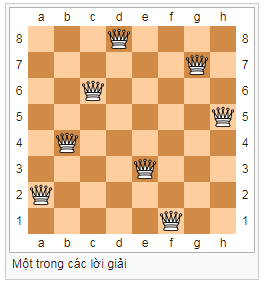
\includegraphics[scale=1]{image/hinhboard8x8}\\[1cm]
%\end{center}

%\subsubsection{Lịch sử}.



%%%%%%%%%%%%%%
\section{Kết Luận }\label{result}
Bài báo cáo đã trình bày một cách tông quát làm sao để phân tích dữ liệu sử dụng môi trường Hadoop MapReduce. Kiến thức trong bài được dựa trên bài báo cáo khoa học " Data analysis using hadoop MapReduce environment" (thông tin bài báo các bạn có thể xem thêm ở đường dẫn sau đây: https://ieeexplore.ieee.org/document/8258541/metrics).

%%%%%%%%%%%%%%
\section{Tài liệu Tham Khảo }
http://en.wikipedia.org\\
https://vi.wikipedia.org/wiki\\
https://ieeexplore.ieee.org/document/8258541/metrics\#metrics\\

%%%%%%%%%%%%%%

\end{document}



